\section{Objective}
\begin{itemize}
	\item To develop practical understanding of charge conservation (Kirchhoff's Current Law) and energy conservation (Kirchhoff's Voltage Law) in electric circuits.
	\item To construct multi-node DC networks and accurately record branch currents and potential drops using a digital multimeter.
	\item To evaluate current distribution at circuit nodes and confirm that loop voltage sums balance to zero.
	\item To compare empirical measurements against theoretical predictions while evaluating potential sources of physical error.
\end{itemize}

\section{Introduction}
Along with Ohm's Law, Kirchhoff's laws provide the foundational framework required to analyze complex linear resistive networks. Kirchhoff's Current Law (KCL) governs the conservation of electrical charge across circuit junctions, whereas Kirchhoff's Voltage Law (KVL) reflects energy conservation along closed loops. This experiment tests both principles using a multi-branch DC network and quantifies differences between theoretical expectations and laboratory multimeter measurements.

\section{Theory}

\subsection{Kirchhoff's Current Law (KCL)}
Kirchhoff's Current Law establishes that the algebraic sum of all currents entering and exiting any node must equal zero:
\[
\sum_{k=1}^{n} I_k = 0,
\]
taking currents entering a junction as positive and currents leaving as negative. Consequently, total current entering a node matches total current leaving it. For a node where main supply current $I$ divides into two parallel branches:
\[
I_{\text{total}} = I_1 + I_2.
\]

\subsection{Kirchhoff's Voltage Law (KVL)}
Kirchhoff's Voltage Law establishes that the algebraic sum of all potential drops and rises along any closed loop equals zero:
\[
\sum_{k=1}^{n} V_k = 0.
\]
When traversing a loop, voltage rises across source terminals are assigned positive values, whereas potential drops across load resistors are negative. For a single loop containing a source $V_S$ and two series resistors, $V_S - V_1 - V_2 = 0$, giving $V_S = V_1 + V_2 = I(R_1+R_2)$.

\section{Apparatus and Components}
\begin{table}[h!]
	\centering
	\caption{List of Equipment and Components Used}
	\vspace{2mm}
	\begin{tabular}{llc}
		\toprule
		\rowcolor{blue!10}
		\textbf{Item Description} & \textbf{Specification / Rating} & \textbf{Quantity} \\
		\midrule
		DC Power Supply & Regulated DC output & 1 \\
		Fixed Resistors & $R_1, R_2, R_3$ (\qty{100}{\ohm}--\qty{330}{\ohm} range) & 3 \\
		Digital Multimeter (DMM) & DC Voltage / Current modes & 1 \\
		Solderless Breadboard & Standard Tie-Point & 1 \\
		Connecting Wires & Jumper Wires & As required \\
		\bottomrule
	\end{tabular}
	\label{tab:apparatus3}
\end{table}

\section{Circuit Diagrams}

\subsection{Circuit for KCL Verification}
\begin{figure}[h!]
	\centering
	\begin{circuitikz}[american, scale=1.0]
		\draw (0,0) to[battery1, invert] (0,3)
		(0,3) to[R, l=$R_1$, i=$I$] (4,3)
		to[R, l=$R_2$, i=$I_1$] (8,3) -- (8,0) -- (0,0);
		\draw (4,3) to[R, l=$R_3$, i_=$I_2$] (4,0);
		\draw (4,0) node[ground]{};
	\end{circuitikz}
	\caption{Circuit setup for KCL verification: source current $I$ divides at the main node into parallel branch currents $I_1$ and $I_2$, giving $I = I_1 + I_2$.}
	\label{fig:kclcircuit}
\end{figure}

\subsection{Circuit for KVL Verification}
\begin{figure}[h!]
	\centering
	\begin{circuitikz}[american, scale=1.0]
		\draw (0,0) to[battery1, l=$V$, invert] (0,3)
		(0,3) to[R, l=$R_1$, v=$V_{R_1}$] (4,3)
		to[R, l=$R_2$, v=$V_{R_2}$] (8,3) -- (8,0) -- (0,0);
		\draw (4,3) to[R, l=$R_3$, v_=$V_{R_3}$] (4,0);
		\draw (4,0) node[ground]{};
		\node at (2,1.7) {Loop 1};
		\node at (6,1.7) {Loop 2};
	\end{circuitikz}
	\caption{Circuit setup for KVL verification: Loop 1 ($R_1$, $R_3$, and $V$) and Loop 2 ($R_2$ and $R_3$) define closed loops.}
	\label{fig:kvlcircuit}
\end{figure}

\section{Experimental Procedure}

\subsection*{Part A: Verification of KCL}
\begin{enumerate}
	\item Assemble the network shown in Figure~\ref{fig:kclcircuit} on the breadboard, connecting the DC power supply through $R_1$ into the junction of $R_2$ and $R_3$.
	\item Configure the DMM to measure DC current and place it in series with the DC source to record total input current $I_{\text{total}}$.
	\item Measure branch currents $I_1$ and $I_2$ individually by inserting the DMM sequentially into series with $R_2$ and $R_3$.
	\item Sum the measured branch currents ($I_1 + I_2$) and compare the total against measured total current $I_{\text{total}}$ and nominal theoretical estimates.
\end{enumerate}

\subsection*{Part B: Verification of KVL}
\begin{enumerate}
	\item Adjust the circuit connections to form the dual-loop setup in Figure~\ref{fig:kvlcircuit}.
	\item Set the DMM to DC voltage measurement mode and record potential drops across every resistor ($V_{R_1}$, $V_{R_2}$, $V_{R_3}$).
	\item Calculate the algebraic sum of voltages for Loop 1 ($V_{R_1} + V_{R_3} - V$) and Loop 2 ($V_{R_2} - V_{R_3}$) to test agreement with zero.
	\item Compare experimental algebraic loops against expected theoretical values.
\end{enumerate}

\section{Data Collection}

\begin{table}[h!]
	\centering
	\caption{Experimental Data for the Verification of KCL}
	\vspace{2mm}
	\begin{tabular}{ccccc}
		\toprule
		\rowcolor{blue!10}
		\textbf{Input Voltage $V$ (V)} & \textbf{$I_1$ (mA)} & \textbf{$I_2$ (mA)} & \textbf{$I_{\text{total}}$ measured (mA)} & \textbf{$I_{\text{total}}$ theoretical (mA)} \\
		\midrule
		10 & 17.23 & 9.9 & 24.4 & 24.814 \\
		\bottomrule
	\end{tabular}
	\label{tab:kcldata}
\end{table}

\begin{table}[h!]
	\centering
	\caption{Experimental Data for the Verification of KVL}
	\vspace{2mm}
	\begin{tabular}{cccccccc}
		\toprule
		\rowcolor{blue!10}
		\textbf{Loop} & \textbf{$V$ (V)} & \textbf{$V_{R_1}$ (V)} & \textbf{$V_{R_2}$ (V)} & \textbf{$V_{R_3}$ (V)} & \textbf{Alg. Sum measured (V)} & \textbf{Alg. Sum theoretical (V)} \\
		\midrule
		1 & 10 & 8.04 & 1.64 & 1.64 & 9.79 & 10.212 \\
		2 & 10 & 4.02 & 0.85 & 0.85 & 5.72 & 5.976 \\
		\bottomrule
	\end{tabular}
	\label{tab:kvldata}
\end{table}

\section{Calculation}
\subsection{KCL Percentage Error}
\[
\text{\% Error (KCL)} = \left| \frac{I_{\text{total(theoretical)}} - I_{\text{total(measured)}}}{I_{\text{total(theoretical)}}} \right| \times 100\%
= \left| \frac{24.814 - 24.4}{24.814} \right| \times 100\% \approx 1.67\%.
\]

\subsection{KVL Percentage Error}
Calculating error across loops yields:
\[
\text{\% Error (KVL)} = \left| \frac{\text{Alg. Sum theoretical} - \text{Alg. Sum measured}}{\text{Alg. Sum theoretical}} \right| \times 100\%.
\]
For Loop 1: $\left|(10.212-9.79)/10.212\right|\times100\% \approx 4.13\%$. For Loop 2: $\left|(5.976-5.72)/5.976\right|\times100\% \approx 4.28\%$.

\section{Result Analysis}
The measured total current ($I_{\text{total}} = \qty{24.4}{\milli\ampere}$) closely matched the calculated value ($\qty{24.814}{\milli\ampere}$), yielding an error of $1.67\%$ and verifying KCL. For KVL, loop voltage sums remained within $4.13\%$ and $4.28\%$ of theoretical targets, confirming energy conservation across closed branches.

\section{Discussion and Sources of Error}
Minor discrepancies between measured and calculated values stem from specific physical factors:
\begin{enumerate}
	\item \textbf{Ammeter Loading:} Non-zero internal resistance inside the multimeter introduces small burden voltages during current measurements.
	\item \textbf{Resistor Tolerances:} Discrepancies between nominal color codes and actual resistance values shift measured currents slightly away from theoretical models.
	\item \textbf{Voltmeter Loading:} Finite internal impedance of the voltmeter draws minor current from measured nodes.
	\item \textbf{Breadboard Contact Resistance:} Interconnection contacts and jumper leads add small parasitic resistances across loop paths.
\end{enumerate}

\section{Conclusion}
Experimental data successfully confirms both Kirchhoff's Current Law and Kirchhoff's Voltage Law within minor error margins. Measured current entering the junction matched the sum of branch currents, and potential changes along closed loops balanced in agreement with theoretical calculations.

\section{References}
\begin{tcolorbox}[colback=gray!5, colframe=gray!40, arc=2mm]
	\begin{enumerate}
		\item Alexander, C. K., \& Sadiku, M. N. O. (2016). \textit{Fundamentals of Electric Circuits} (6th ed.). McGraw-Hill Education.
		\item Hayt, W. H., Kemmerly, J. E., \& Durbin, S. M. (2012). \textit{Engineering Circuit Analysis} (8th ed.). McGraw-Hill Education.
		\item Boylestad, R. L. (2015). \textit{Introductory Circuit Analysis} (13th ed.). Pearson.
	\end{enumerate}
\end{tcolorbox}

\section{Lab Data Sheet}
\begin{center}
	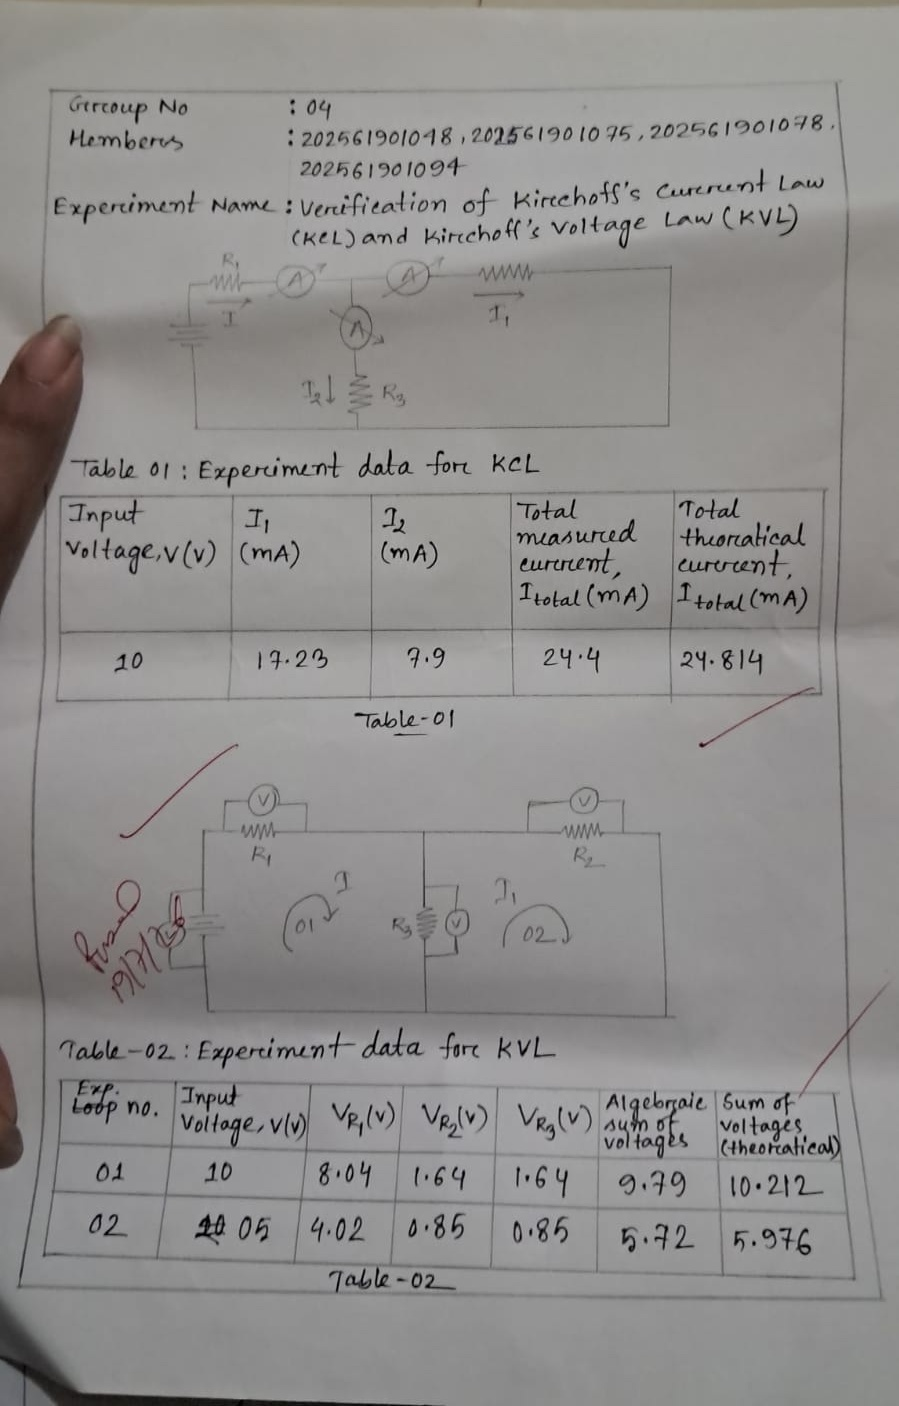
\includegraphics[width=0.95\textwidth, height=0.70\textheight, keepaspectratio]{datasheet1.png}
	
	\vspace{2mm}
	\small\textbf{Figure 3: Handwritten Lab Data Sheet for Experiment 03}
\end{center}